\section{}
\[
H(s)=\frac{s+1}{s+10}\,.
\]
\subsection{Bode-Diagramm}
\begin{center}
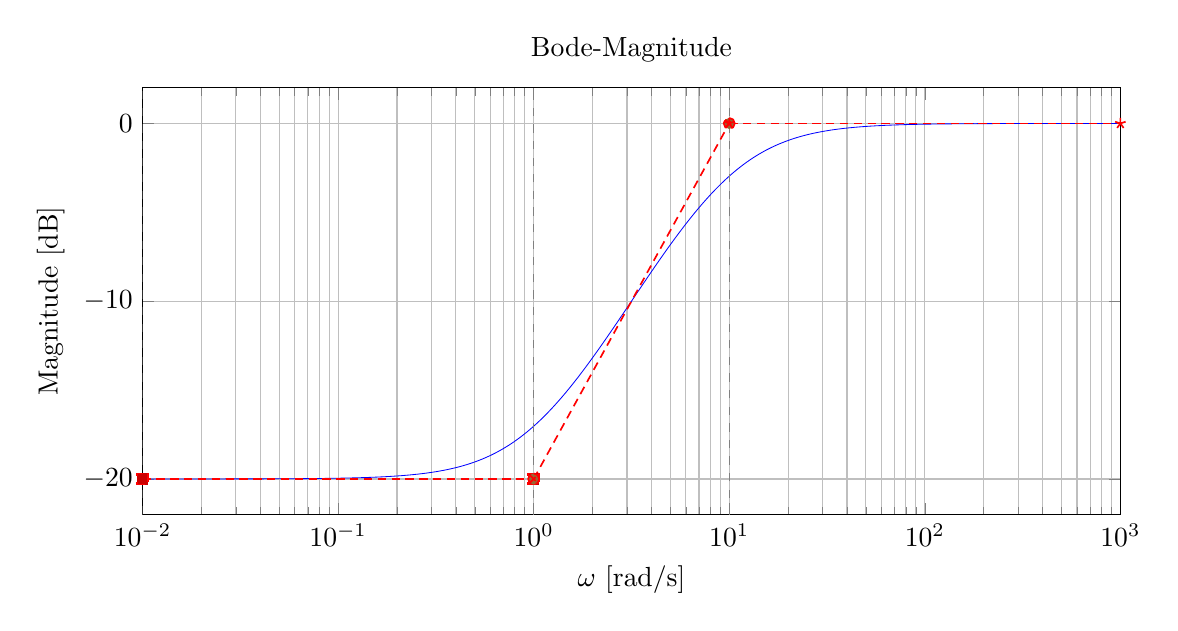
\begin{tikzpicture}
\begin{semilogxaxis}[
  width=14cm,height=7cm,
  xmin=1e-2,xmax=1e3,
  xlabel={$\omega$ [rad/s]},
  ylabel={Magnitude [dB]},
  grid=both,
  ytick distance=10,
  title={Bode-Magnitude}
]
\addplot[
  domain=1e-2:1e3,
  samples=600,
  mark=none,
  line width=0.3pt,
  blue
] {20*ln(sqrt(1 + x^2))/ln(10) - 20*ln(sqrt(100 + x^2))/ln(10)};
\addplot+[domain=1e-2:1,samples=2,dashed,dash pattern=on 3pt off 2pt,line width=0.6pt,red] {-20};
\addplot+[domain=1:1e1,samples=2,dashed,dash pattern=on 3pt off 2pt,line width=0.6pt,red] {-20 + 20*ln(x)/ln(10)};
\addplot+[domain=1e1:1e3,samples=2,dashed,dash pattern=on 3pt off 2pt,line width=0.6pt,red] {0};
\draw[gray,dashed] (rel axis cs:0,0) -- (rel axis cs:0,1);
\draw[gray,dashed] (axis cs:1,\pgfkeysvalueof{/pgfplots/ymin}) -- (axis cs:1,\pgfkeysvalueof{/pgfplots/ymax});
\draw[gray,dashed] (axis cs:10,\pgfkeysvalueof{/pgfplots/ymin}) -- (axis cs:10,\pgfkeysvalueof{/pgfplots/ymax});
\node[gray,anchor=south east] at (axis cs:1,\pgfkeysvalueof{/pgfplots/ymax}) {\scriptsize Nullstelle $\omega_z=1$};
\node[gray,anchor=south east] at (axis cs:10,\pgfkeysvalueof{/pgfplots/ymax}) {\scriptsize Pol $\omega_p=10$};
\end{semilogxaxis}
\end{tikzpicture}
\vspace{6mm}
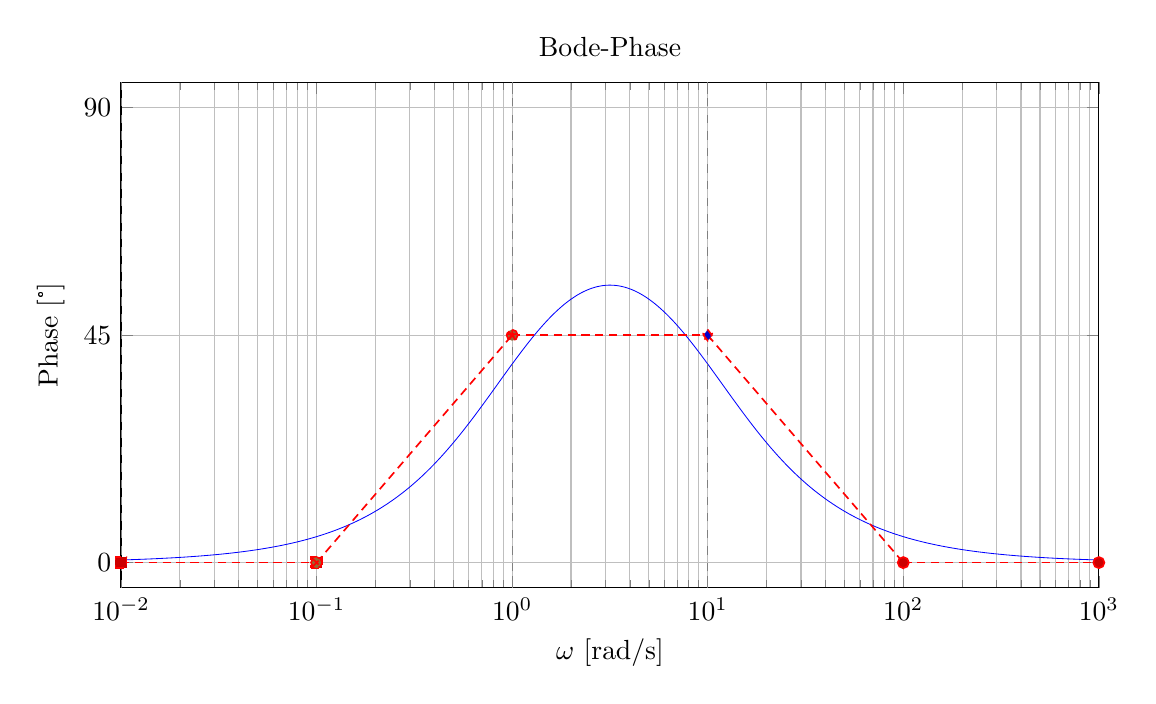
\begin{tikzpicture}
\begin{semilogxaxis}[
  width=14cm,height=8cm,
  xmin=1e-2,xmax=1e3,
  ymin=-5,ymax=95,
  ytick distance=45,
  xlabel={$\omega$ [rad/s]},
  ylabel={Phase [°]},
  grid=both,
  title={Bode-Phase}
]
\addplot[
  domain=1e-2:1e3,
  samples=600,
  mark=none,
  line width=0.3pt,
  blue
] {atan(x) - atan(x/10)};
\addplot+[domain=1e-2:1e-1,samples=2,dashed,dash pattern=on 3pt off 2pt,line width=0.6pt,red] {0};
\addplot+[domain=1e-1:1e0,samples=2,dashed,dash pattern=on 3pt off 2pt,line width=0.6pt,red] {45 + 45*ln(x)/ln(10)};
\addplot+[domain=1e0:1e1,samples=2,dashed,dash pattern=on 3pt off 2pt,line width=0.6pt,red] {45};
\addplot+[domain=1e1:1e2,samples=2,dashed,dash pattern=on 3pt off 2pt,line width=0.6pt,red] {45 - 45*ln(x/10)/ln(10)};
\addplot+[domain=1e2:1e3,samples=2,dashed,dash pattern=on 3pt off 2pt,line width=0.6pt,red] {0};
\draw[gray,dashed] (rel axis cs:0,0) -- (rel axis cs:0,1);
\draw[gray,dashed] (axis cs:1,\pgfkeysvalueof{/pgfplots/ymin}) -- (axis cs:1,\pgfkeysvalueof{/pgfplots/ymax});
\draw[gray,dashed] (axis cs:10,\pgfkeysvalueof{/pgfplots/ymin}) -- (axis cs:10,\pgfkeysvalueof{/pgfplots/ymax});
\node[gray,anchor=south east] at (axis cs:1,\pgfkeysvalueof{/pgfplots/ymax}) {\scriptsize Nullstelle $\omega_z=1$};
\node[gray,anchor=south east] at (axis cs:10,\pgfkeysvalueof{/pgfplots/ymax}) {\scriptsize Pol $\omega_p=10$};
\end{semilogxaxis}
\end{tikzpicture}
\end{center}
\newpage
\subsection{Erklärung}
\begin{description}[leftmargin=1.2em,labelsep=.6em,font=\bfseries]

\item[1. Zuerst Normalform herstellen.]
\[
H(s)=\frac{s+1}{s+10}=\frac{1+sT_z}{10\,(1+sT_p)}
\]
Die Teilglieder und Variablen gemäß Skript sind: 
\[
\underline{F}_1(s)=\frac{1}{1+s\frac{1}{10}},\; \underline{F}_2(s)=1+s,\quad T_z=1,\;T_p=\tfrac{1}{10},\;K_0=\tfrac{1}{10}\;\text{und}\;r=0.
\]

reelle Nullstelle erster Ordnung bei $\omega_z=1/T_z=1 \,\mathrm{rad/s}$; reeller Pol erster Ordnung bei $\omega_p=1/T_p=10\,\mathrm{rad/s}$.

\item[2. Danach Eckfrequenzen bestimmen und sortieren.]
\[
\omega_z=1\,\mathrm{rad/s},\qquad \omega_p=10\,\mathrm{rad/s},\qquad \omega_z<\omega_p.
\]

\item[3. Startpunkt des Amplitudengangs (Geradennäherung).]
Setze $\omega_{\min}=\omega_z=1$.
\[
F_{\mathrm{dB}}(\omega_{\min})=20\log_{10}\!\big(|K_0\,F^*_{ges}(0)|\,\omega_{\min}^{\,r}\big)
=20\log_{10}\!\big(\tfrac{1}{10}\big)=-20\,\mathrm{dB}.
\]
Anfangssteigung $r\cdot 20\,\mathrm{dB/dec}=0$.

\item[4. Verlauf links vom Startpunkt.]
Für $\omega<1$ bleibt die Magnitude-Asymptote horizontal bei $-20\,\mathrm{dB}$, da $r=0$.

\item[5. Steigungswechsel an den Ecken.]
Die Nullstelle bei $\omega_z=1$ erhöht die Steigung um $+20\,\mathrm{dB/dec}$.
Der Pol bei $\omega_p=10$ senkt sie wieder um $-20\,\mathrm{dB/dec}$.
Damit:
\[
\begin{cases}
\omega<1:\ \ 0\,\mathrm{dB/dec},\\
1\le\omega<10:\ \ +20\,\mathrm{dB/dec},\\
\omega\ge10:\ \ 0\,\mathrm{dB/dec}.
\end{cases}
\]

\item[6. Eckabrundung (exakte Stützpunkte).]
\[
|H(j\omega)|=\frac{\sqrt{1+\omega^2}}{\sqrt{100+\omega^2}},\qquad
|H(j\cdot 1)|_{\mathrm{dB}}=10\log_{10}\!\Big(\frac{2}{101}\Big)\approx -17.03\,\mathrm{dB},
\]
\[
|H(j\cdot 10)|_{\mathrm{dB}}=10\log_{10}\!\Big(\frac{101}{200}\Big)\approx -2.97\,\mathrm{dB}.
\]
Bei $\omega=1$ liegt die Kurve $\approx 3\,\mathrm{dB}$ über der Geradennäherung, bei $\omega=10$ $\approx 3\,\mathrm{dB}$ darunter. Auch hier gilt: Mehrfachpole/-nullstellen sorgen für eine Rundung um $t\cdot3\,\mathrm{dB}$

\item[7. Phasenstartwert.]
Da $K_0F_{ges}(0) >0$ gilt:
\[
\varphi(0)=r\cdot 90^\circ = 0^\circ.
\]

\item[8. Phasenänderung durch Nullstelle und Pol.]
Reelle Nullstelle 1.\,Ordnung: $0^\circ\to +90^\circ$ über $[0.1,10]$.
Reeller Pol 1.\,Ordnung: $0^\circ\to -90^\circ$ über $[1,100]$. Die Phasensteigungs und -senkungseffekte überschneiden sich in $[10,100]$ und addieren sich dort. In diesem Interval bleibt also die Phase gleich
Die Geradennäherung lautet also:
\[
\varphi(\omega)\approx
\begin{cases}
0^\circ,& \omega\le 0.1,\\
+45^\circ+45^\circ\log_{10}\omega,& 0.1<\omega<1,\\
+45^\circ,& 1\le\omega\le 10,\\
+45^\circ-45^\circ\log_{10}(\omega/10),& 10<\omega<100,\\
0^\circ,& \omega\ge 100.
\end{cases}
\]

\item[9. Exakte Stützstellen (Kontrolle).]
\[
\varphi(\omega)=\arctan(\omega)-\arctan\!\Big(\frac{\omega}{10}\Big)\,[^\circ].
\]
Praktische Punkte:
\[
\begin{aligned}
\omega=0.1:&\quad |H|_{\mathrm{dB}}\approx -19.96,\ \ \varphi\approx +5.14^\circ,\\
\omega=1:&\quad |H|_{\mathrm{dB}}\approx -17.03,\ \ \varphi\approx +39.29^\circ,\\
\omega=10:&\quad |H|_{\mathrm{dB}}\approx -2.97,\ \ \varphi\approx +39.29^\circ,\\
\omega=100:&\quad |H|_{\mathrm{dB}}\approx -0.04,\ \ \varphi\approx +5.14^\circ.
\end{aligned}
\]

\item[10. Grenzwerte und Konsistenz.]
DC: $|H(0)|=\tfrac{1}{10}\Rightarrow -20\,\mathrm{dB}$, $\varphi(0)=0^\circ$.
Für $\omega \to \infty$: $|H(j\omega)|\to 1\Rightarrow 0\,\mathrm{dB}$.
Pol-/Nullzählung: $m=n=1\Rightarrow \varphi(\infty)=(m-n)\cdot90^\circ=0^\circ$.
\end{description}

\newpage